\documentclass[11pt]{article}
\title{\textbf{Meccano frames}}
\author{https://github.com/heptagons/meccano/frames}
\date{}

\usepackage{../meccano}
\usepackage{tikz}
\usetikzlibrary{calc}
\usepackage{ifthen}

\newcommand{\meccanoframetriangleextra}[3]{
 \def\dd{#1}
 \def\ff{#2}
 \def\gg{#3}
 \ifthenelse{\ff=0 \OR \gg=0}{}{
  \pgfmathsetmacro{\cosf}{(#1^2 + #2^2 - #3^2)/(2*#1*#2)} % (d^2 + f^2 - g^2)/(2df)
  \begin{scope}[shift={(\dd,0)},rotate={180-acos(\cosf)}]
   \meccanostrip[cc0000]{\ff}{1}{\p}
  \end{scope}
  \pgfmathsetmacro{\cosg}{(#1^2 + #3^2 - #2^2)/(2*#1*#3)} % (d^2 + g^2 - f^2)/(2dg)
  \begin{scope}[rotate={acos(\cosg)}]
   \meccanostrip[cc0000]{\gg}{1}{\p}
   \path (\gg,0) ++(0:5*\p) node{$F$};
  \end{scope}


  %\path (0,0) ++(90:10*\p) node{$\ff$};
 }
}

\newcommand{\meccanoframetriangle}[9]{%a,b,c,d,e,p,scale, f,g
\begin{tikzpicture}
\def\p{#6}
\def\f{#8}
\def\g{#9}
\pgfmathsetmacro{\ad}{#1 + #4} % a+d
\pgfmathsetmacro{\be}{#2 + #5} % b+e
\pgfmathsetmacro{\cosb}{(#1^2 + #3^2 - #2^2)/(2*#1*#3)} % (a^2 + c^2 - b^2)/(2ac)
\pgfmathsetmacro{\cosa}{(#2^2 + #3^2 - #1^2)/(2*#2*#3)} % (b^2 + c^2 - a^2)/(2bc)
\begin{scope}[scale=#7]
  \meccanostrip[0000cc]{#3}{1}{\p} % blue c=BA
   \begin{scope}[rotate={acos(\cosb)},shift={(-#4,0)}] % shift -d
    \meccanostrip[cc0000]{\ad}{1}{\p} % red a+d=CB+BE
    \path (0,0) ++(180:5*\p) node{$E$};
    \path (#4,0) ++(90:5*\p) node{$B$}; %d
    \path (\ad,0) ++(90:5*\p) node{$C$};
    \meccanoframetriangleextra{\ad}{\f}{\g} % d,f,g
   \end{scope}
   \begin{scope}[shift={(#3,0)},rotate=180-acos{\cosa},shift={(-#5,0)}] % shift c, shift -e
    \meccanostrip[008800]{\be}{1}{\p} % green b+e=CA+AD
    \path (#5,0) ++(-90:5*\p) node{$A$}; %e
    \path (0,0) ++(-180:5*\p) node{$D$};
   \end{scope}
\end{scope}
\end{tikzpicture}
}

\newcommand{\meccanoframefive}[8]{ %a,b,c,d,e, p,scale, x+g, g,h,i,j,k, x
\begin{tikzpicture}
\def\p{#6}
\def\xg{#8}
\pgfmathsetmacro{\ad}{#1 + #4} % a+d
\pgfmathsetmacro{\be}{#2 + #5} % b+e
\pgfmathsetmacro{\cosb}{(#1^2 + #3^2 - #2^2)/(2*#1*#3)} % (a^2 + c^2 - b^2)/(2ac)
\pgfmathsetmacro{\cosa}{(#2^2 + #3^2 - #1^2)/(2*#2*#3)} % (b^2 + c^2 - a^2)/(2bc)
\pgfmathsetmacro{\x}{max(#3,\xg)} % max(c,x+g)
\begin{scope}[scale=#7] 
 \path (0,0) ++(180:5*\p) node{$A$};
 \meccanostrip[0000cc]{\x}{1}{\p}
 \begin{scope}[rotate={acos(\cosb)}]
  \meccanostrip[cc0000]{\ad}{1}{\p} % red a+d=CB+BE
  \path(#3,0) ++(-45:5*\p) node{$C$};
  \path(\ad,0) ++(0:5*\p) node{$D$};
 \end{scope}
 \begin{scope}[shift={(#3,0)},rotate=180-acos{\cosa}] % shift \c
  \meccanostrip[008800]{\be}{1}{\p} % green b+e=CA+AD
  \path(0,0) ++(-90:5*\p) node{$B$};
  \path(\be,0) ++(0:5*\p) node{$E$};
 \end{scope}
 \meccanoframefivebelow
}

\newcommand{\meccanoframefivebelow}[6]{ % g,h,i,j,k, x
\def\x{#6}
\pgfmathsetmacro{\gj}{#1 + #4} % g+j
\pgfmathsetmacro{\hk}{#2 + #5} % h+k
\pgfmathsetmacro{\cosb}{(#1^2 + #3^2 - #2^2)/(2*#1*#3)} % (a^2 + c^2 - b^2)/(2ac)
\pgfmathsetmacro{\cosg}{(#2^2 + #3^2 - #1^2)/(2*#2*#3)} % (b^2 + c^2 - a^2)/(2bc)
 \begin{scope}[shift={(\x,0)},rotate={-acos(\cosg)}]
  \meccanostrip[cc00cc]{\gj}{1}{\p}
  \path (0,0) ++(180:5*\p) node{$G$};
  \path (#3,0) ++(45:5*\p) node{$I$};
  \path (\gj,0) ++(0:5*\p) node{$K$};
 \end{scope}
 \begin{scope}[shift={(\x+#3,0)},rotate={180+acos(\cosb)}]
  \meccanostrip[cc8800]{\hk}{1}{\p}
  \path (0,0) ++(180:5*\p) node{$H$};
  \path (\hk,0) ++(0:5*\p) node{$J$};
 \end{scope}

\end{scope} %above
\end{tikzpicture} %above
}


\begin{document}

\maketitle
\begin{abstract}
Meccano frames are groups of meccano\meccanoref strips intended to be a
base to build diverse meccano larger objects.
\end{abstract}

\section{Triangular frame}

\begin{figure}[h]
\centering
\meccanoframetriangle{5}{4}{7}{3}{1}{3pt}{0.75}{0}{0}
\caption{Triangular frame. With three strips we form the triangle $\triangle{ABC}$.
At least we extend one of two strips $\overline{CB}$ and $\overline{CA}$ to become
$\overline{CE}$ and $\overline{CD}$. The new vertices $D$ and $E$ are rigid as the
triangle and we'll calculate the distance between them which most of the time is not longer an integer.}
\label{fig:triangle}
\end{figure}

Figure \ref{fig:triangle} shows the three strips triangular frame with extensions. 
First we identify five integer distances $a,b,c,d,e$:
\begin{align}
a &\equiv \overline{CB},\quad b \equiv \overline{CA},\quad c \equiv \overline{AB},\quad c < a+b\\
d &\equiv \overline{CB} + \overline{BE} = \overline{CE} \geq a \\
e &\equiv \overline{CA} + \overline{AD} = \overline{CD} \geq b
\end{align}

We calculate the cosine of $\angle{BCA}$:
\begin{align}
\theta &\equiv \angle{BCA} \\
\cos\theta &= \frac{a^2 + b^2 - c^2}{2ab}
\end{align}
Then we apply the cosine to the triangle $\triangle{CED}$ to get the
extensions distance $\overline{DE}$:
\begin{align}
\overline{DE}^2 &= \overline{CD}^2 + \overline{CE}^2
 - 2\overline{CD} \times \overline{CE}\cos\theta \nonumber\\
 &= d^2 + e^2 - 2de\cos\theta \nonumber\\
 &= d^2 + e^2 - de\left(\frac{a^2 + b^2 - c^2}{ab}\right)
\end{align}
We expect at most a value of the form $\sqrt{s}/t$ where $s, t \in \bbb{Z^+}$
so we define the surd as:
\begin{align}
 \overline{DE} &= \sqrt{d^2 + e^2 - de\left(\frac{a^2 + b^2 - c^2}{ab}\right)}\nonumber\\
 &= \frac{\sqrt{a^2b^2(d^2 + e^2) - abde(a^2 + b^2 - c^2)}}{ab}\nonumber\\
 &= \frac{\sqrt{ab((ad-be)(bd-ae)+c^2de)}}{ab} \nonumber\\
 &= \frac{\sqrt{s}}{t}\\
 t &= ab \\
 s &= t((ad-be)(bd-ae)+c^2de)
\end{align}

\subsection{Rigid distances $\sqrt{s}$ and $\sqrt{s} + f$}

\begin{figure}[h]
\centering
\begin{center}
\meccanoframetriangle{1}{1}{1}{0}{2}{3pt}{1.0}{0}{0}(a)
\meccanoframetriangle{3}{2}{2}{0}{2}{3pt}{0.7}{5}{4}(b)\qquad
\meccanoframetriangle{4}{4}{1}{2}{4}{3pt}{0.6}{0}{0}(c)\qquad
\meccanoframetriangle{7}{5}{3}{0}{2}{3pt}{0.6}{0}{0}(d)
\end{center}
\caption{Four frames with rigid distance $\overline{DE}=\sqrt{7}$ reported by
the factory software mentioned in this section. The particular case (b),
was reported with the angle $CED=\pi/2$ which means we can append two extra strips to make
a pythagorean triangle $\triangle{CEF}$ where angle ${CEF}=\pi/2$, which makes
the three vertices $D,E,F$ collinear, so the rigid distance $\overline{DF}=\sqrt{7}+4$ is an algebraic number.
}
\label{fig:surd7}
\end{figure}

We write a factory to report all the triangles with specific surd $\sqrt{s}$
for a given maximum strips length.
We reject $t \neq 1$ and $s$ as not square-free, which includes pythagorean triangles.
Next list show all the triangles with $s = \sqrt{7}, t=1$ where
$c < a+b$, $a\leq d\leq max$, $b\leq e\leq max$, $c\leq max$:
\begin{lstlisting}
=== RUN   TestFramesTriangleSurds
NewFrames().TriangleSurds surd=7 max=15
  1) a=1 e=1+2 c=1 cos=1/2
  2) d=1+1 e=1+2 c=1 cos=1/2
  3) d=1+2 b=1 c=1 cos=1/2
  4) d=1+2 e=1+1 c=1 cos=1/2
  5) a=2 e=2+1 c=2 cos=1/2
  6) d=2+1 b=2 c=2 cos=1/2
  7) a=3 e=2+2 c=2 cos=3/4 CED=pi/2
  8) d=3+1 e=2+1 c=2 cos=3/4 CDE=pi/2
  9) d=4+2 e=4+4 c=1 cos=31/32
 10) d=4+4 e=4+2 c=1 cos=31/32
 11) a=7 e=5+1 c=3 cos=13/14
 12) a=7 e=5+2 c=3 cos=13/14
\end{lstlisting}
Figure \ref{fig:surd7} show four cases of this list.
The code is in the folder \texttt{github.com/heptagons/meccano/frames}.



\section{More rigid distances $\sqrt{s} + h$}

We explore a more complicated frame to get additional cases of distances $\sqrt{s} + h$ without
relying in an explicit pythagorean triangle as we saw in case (b) of figure \ref{fig:surd7}.

\begin{figure}[h]
\centering
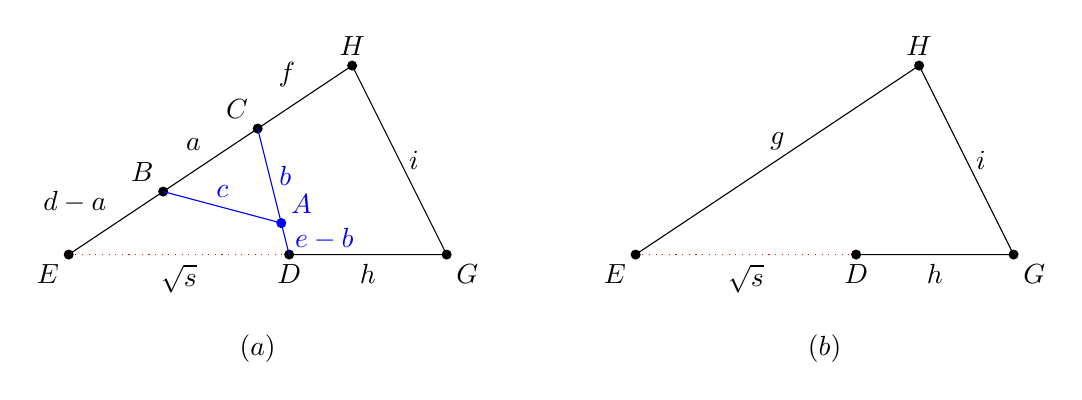
\begin{tikzpicture}
\begin{scope}[scale=0.4]
\begin{scope}
\draw[red,dotted] (0,0) -- node[below,black]{$\sqrt{s}$}++(7,0);
\draw[black,fill=black] (7,0) node[below]{$D$}  circle(4pt)
-- node[below]{$h$} ++(5,0) node[below right]{$G$} circle(4pt)
-- node[right]{$i$} ++(-3,6) node[above]{$H$} circle(4pt)
-- node[above left]{$f$} ++(-3,-2) node[above left]{$C$} circle(4pt)
-- node[above left]{$a$} ++(-3,-2) node[above left]{$B$} circle(4pt)
-- node[above left]{$d-a$} ++(-3,-2) node[below left]{$E$} circle(4pt);
\draw[blue,fill=blue] (7,0)
-- node[right]{$e-b$} ++(-.25,1) node[above right]{$A$} circle(4pt)
-- node[right]{$b$} ++(-.75,3)
   ++(+.75,-3)
-- node[above]{$c$} (3,2);
\draw[black](6,-3) node{$(a)$};
\end{scope}

\begin{scope}[shift={(18,0)}]
\draw[red,dotted] (0,0) -- node[below,black]{$\sqrt{s}$}++(7,0);
\draw[black,fill=black] (7,0) node[below]{$D$}  circle(4pt)
-- node[below]{$h$} ++(5,0) node[below right]{$G$} circle(4pt)
-- node[right]{$i$} ++(-3,6) node[above]{$H$} circle(4pt)
-- node[above]{$g$} ++(-9,-6) node[below left]{$E$} circle(4pt);
\draw[black](6,-3) node{$(b)$};
\end{scope}


\end{scope}
\end{tikzpicture}
\caption{The five strips intented to form an algebraic distance $\overline{EG} = \sqrt{s} + h$.}
\label{fig:alg-not-right}
\end{figure}

From figure \ref{fig:alg-not-right} $(a)$ we know $\sqrt{s}$ distance
between nodes $E$ and $D$ is produced by the three strips frame $a+d$, $b+e$ and $c$.
Using the law of cosines we calculate the angle $\theta = \angle{CED}$ in terms of $\sqrt{s}$:

\begin{align}
\cos\theta &= \frac{d^2 + (\sqrt{s})^2 - e^2}{2d\sqrt{s}} \nonumber\\
 &= \frac{(d^2 + s - e^2)\sqrt{s}}{2ds} \\
 &= \frac{m\sqrt{s}}{n} \label{eq:cos1}\\
 m &= d^2 + s - e^2 \\
 n &= 2ds
\end{align}

From figure \ref{fig:alg-not-right} $(a)$ we notice two sets of points are collinear:
$\{ E,B,C,H \}$ and $\{ E,D,G \}$. Using the law of cosines we calculate the 
angle $\theta = \angle{HEG}$ in terms of distances $g,\sqrt{s}+h,i$:

\begin{align}
\cos\theta &= \frac{g^2 + (\sqrt{s}+h)^2 - i^2}{2g(\sqrt{s}+h)} \nonumber\\
 &= \frac{g^2 + s + 2\sqrt{s}h + h^2 - i^2}{2g(\sqrt{s}+h)} \nonumber\\
 &= \frac{g^2 + s + h^2 - i^2+ 2\sqrt{s}h}{2g(\sqrt{s}+h)}
\end{align}

We multiply both numerator and denominator by $\sqrt{s}-h$ to eliminate the surd from denominator:
\begin{align}
\cos\theta &= \frac{(s + g^2 + h^2 - i^2)(\sqrt{s}-h) + 2\sqrt{s}h(\sqrt{s}-h)}
	{2g(\sqrt{s}+h)(\sqrt{s}-h)} \nonumber\\
 &= \frac{(s + g^2 + h^2 - i^2)(\sqrt{s}-h) + 2sh - 2\sqrt{s}h^2}
	{2g(s-h^2)} \nonumber\\ 
 &= \frac{-h(s + g^2 + h^2 - i^2 - 2s) + (s + g^2 + h^2 - i^2 - 2h^2)\sqrt{s}}
	{2g(s-h^2)} \nonumber\\ 
 &= \frac{h(s - g^2 - h^2 + i^2) + (s + g^2 - h^2 - i^2)\sqrt{s}}
	{2g(s-h^2)} \nonumber\\ 
 &= \frac{o + p\sqrt{s}}{q} \label{eq:cos2}\\
o &= h(s - g^2 - h^2 + i^2) \\
p &= s + g^2 - h^2 - i^2 \\
q &= 2g(s-h^2)
\end{align}

We compare both cosines equations \ref{eq:cos1} and \ref{eq:cos2}:
\begin{align}
\frac{m\sqrt{s}}{n} &= \frac{o + p\sqrt{s}}{q}
\end{align}
Since all variables are integers we need two conditions. First $o$ should be zero.
And second $\frac{m}{n} = \frac{p}{q}$.

For condition 1, we force $o$ to be zero:
\begin{align}
o &= 0 \nonumber\\
h(s - g^2 - h^2 + i^2) & = 0 \nonumber\\
s &= g^2 + h^2 - i^2 \label{eq:condition1}
\end{align}

For condition2, we force $m,n,p,q$ as:
\begin{align}
\frac{m}{n} &= \frac{p}{q} \nonumber\\
\frac{d^2 + s - e^2}{2ds} &= \frac{s + g^2 - h^2 - i^2}{2g(s-h^2)} \nonumber\\
\end{align}

We replace the value of $s$ of last equation RHS with the value of equation \ref{eq:condition1}
of condition 1:
\begin{align}
\frac{d^2 - e^2 + s}{ds} &= \frac{s + g^2 - h^2 - i^2}{g(s-h^2)} \nonumber\\
 &= \frac{g^2 + h^2 - i^2 + g^2 - h^2 - i^2}{g(g^2 + h^2 - i^2-h^2)} \nonumber\\
 &= \frac{2(g^2 - i^2)}{g(g^2 - i^2)} \nonumber\\
 &= \frac{2}{g} \nonumber\\
(d^2 - e^2 + s)g &= 2ds \label{eq:condition2}
\end{align}

\boxed{TODO: Examples!!!}


\section{Five strips frame}

\begin{figure}[H]
\centering
% a,b,c,d,e,p,scale, x+g, g,h,i,j,k, x,p
\meccanoframefive{5}{6}{5}{2}{3}{3pt}{0.66} {7} {3}{4}{4}{3}{2} {3}
\caption{Five strips frame. We construct two triangles $\triangle{ABC}$ and
$\triangle{GHI}$. Extending the strips we get four vertices $E,D,J,K$ which
can form four rigid distances of surd type: $\overline{DJ}, \overline{DK},
\overline{EJ}, \overline{EK}$.}
\label{fig:5strips}
\end{figure}

Figure \ref{fig:5strips} shows a frame with five strips. The frame has eleven variables:
\begin{align}
a &= \overline{BC}, \quad b = \overline{AC}, \quad c = \overline{AB}\\
d &= \overline{AD}, \quad e = \overline{AE}\\
f &= \overline{AG}\\
g &= \overline{HI}, \quad h = \overline{GI}, \quad i = \overline{GH}\\
j &= \overline{HJ}, \quad k = \overline{HK}
\end{align}

Assume vertex A is at the origin.
Let $\alpha = \angle{BAC}$, and $D_x,D_y$ the abscissa and orditate of vertex $D$ so we have:
\begin{align}
t &\equiv b^2 + c^2 - a^2\\
x &\equiv 4b^2c^2 - t^2\\
\cos\alpha &= \frac{t}{2bc}\\
\sin\alpha &= \frac{\sqrt{x}}{2bc}\\
D_x &= d\sin\alpha = \frac{d\sqrt{x}}{2bc}\\
D_y &= d\cos\alpha = \frac{dt}{2bc}\\
D_x^2 + D_y^2 &= d^2
\end{align}
Let $\delta = \angle{HGI}$ and $K_x,K_y$ the abscissa and ordinate of
vertex $K$ so we have:
\begin{align}
v &\equiv h^2 + i^2 - g^2\\
y &\equiv 4h^2i^2 - v^2\\
\cos\delta &= \frac{v}{2hi}\\
\sin\delta &= \frac{\sqrt{y}}{2hi}\\
K_x &= f + k\sin\delta = f + \frac{k\sqrt{y}}{2hi}\\
K_y &= -k\cos\delta = -\frac{kv}{2hi}\\
K_x^2 + K_y^2 &= f^2 + 2fk\sin\delta + k^2\\
 &= f^2+k^2 + \frac{fk\sqrt{y}}{hi}
\end{align}
We calculate the distance $\overline{DK}$:
\begin{align}
\overline{DK}^2 &= (D_x+K_x)^2 + (D_y+K_y)^2 \nonumber\\
 &= D_x^2 + 2D_xK_x + K_x^2 + D_y^2 + 2D_yK_y + K_y^2 \nonumber\\
 &= (D_x^2+D_y^2) + (K_x^2+K_y^2) + 2D_xK_x + 2D_yK_y \nonumber\\
 &= d^2 + f^2 + k^2 + \frac{fk\sqrt{y}}{hi}
  + 2\left(\frac{d\sqrt{x}}{2bc}\right)\left(f + \frac{k\sqrt{y}}{2hi}\right)
  + 2\left(\frac{dt}{2bc}\right)\left(-\frac{kv}{2hi}\right) \nonumber\\
 &= d^2 + f^2 + k^2 - \frac{dtkv}{2bchi} + \frac{fk\sqrt{y}}{hi}
  + \frac{df\sqrt{x}}{bc} + \frac{dk\sqrt{xy}}{2bchi}
\end{align}

\end{document}